% vim: ts=4 sts=4 sw=4 et tw=75
\chapter{Portability}
\label{chap:portability}
\begin{quote}
    Finally, standardization, like convention, can be another manifestation
    (证明) of the strong older. But unlike convention it has been accepted
    in Modern architecture as an enriching (丰富) product of our
    technology, yet dreaded (可怕的) for its potential domination and
    brutality.
\end{quote}
\begin{quotesrc}
    Robert Venturi, \bookname{Complexity and Contradiction (矛盾) in
Architecture}
\end{quotesrc}

It's hard to write software that runs correctly and efficiently. So once a
program works in one environment, you don't want to repeat much of the
effort if you move it to a different compiler or processor or operating
system. Ideally (理想地), it should need no changes whatsoever (无论什么).

This ideal is called \emph{portability}. In practice, "portability" more
often stands for the weaker concept that it will be easier to modify the
program as it moves than to rewrite it from scratch (擦除). The less
revision it needs, the more portable it is.

You may wonder why we worry about portability at all. If software is going
to run in only one environment, under specified conditions, why spend time
giving it broader applicability? First, any successful program, almost by
definition, gets used in unexpected ways and unexpected places. Building
software to be more general than its original specification will result in
less maintenance and more utility down the road. Second, environments
change. When the compiler or operating system or hardware is upgraded,
features may change. The less the program depends on special features, the
less likely it is to break and the more easily it will adapt to changing
circumstances. Finally, and most important, a portable program is a better
program. The effort invested to make a program portable also makes it
better designed, better constructed, and more thoroughly tested. The
techniques of portable programming are closely related to the techniques of
good programming in general.

Of course the degree of portability must be tempered (调和) by reality.
There is no such thing as an absolutely portable program, only a program
that hasn't yet been tried in enough environments. But we can keep
portability as our goal by aiming towards software that runs without change
almost everywhere. Even if this goal isn't met completely, time spent on
portability as the program is created will pay off when the software must
be updated.

Our message is this: try to write software that works within the
intersection of the various standards, interfaces and environments it must
accommodate. Don't fix every portability problem by adding special code;
instead, adapt the software to work within the new constraints. Use
abstraction and encapsulation to restrict and control unavoidable
non-portable code. By staying within the intersection of constraints and by
localizing (局部化) system dependencies, your code will become cleaner and
more general as it is ported (移值).

\section{Language}
\label{sec:language}

\emph{Stick to the standard.} The first step to portable code is of course
to program in a high-level language, and within the language standard if
there is one.  Binaries don't port well, but source code does. Even so, the
way that a compiler translates a program into machine instructions is not
precisely defined, even for standard languages.  Few languages in wide use
have only a single implementation; there are usually multiple suppliers,
or versions for different operating systems, or releases that have evolved
over time. How they interpret your source code will vary.

Why isn't a standard a strict definition? Sometimes a standard is
incomplete and fails to define the behavior when features interact
(互相干扰). Sometimes it's deliberately (故意地) indefinite (不确定); for
example, the \verb'char' type in C and C++ may be signed or unsigned, and
need not even have exactly 8 bits. Leaving such issues up to the compiler
writer may allow more efficient implementations and avoid restricting the
hardware the language will run on, at the risk of making life harder for
programmers. Politics and technical compatibility issues may lead to
compromises that leave details unspecified.  Finally, languages are
intricate (复杂的) and compilers are complex; there will be errors in the
interpretation and bugs in the implementation.

Sometimes the languages aren't standardized at all. C has an official
ANSI/ISO standard issued in 1988, but the ISO C++ standard was ratified
(批准) only in 1998; at the time we are writing this, not all compilers in
use support the official definition. Java is new and still years away from
standardization. A language standard is usually developed only after the
language has a variety of conflicting (互相矛盾的) implementations to unify
(统一), and is in wide enough use to justify the expense of
standardization.  In the meantime, there are still programs to write and
multiple environments to support.

So although reference manuals and standards give the impression (印象) of
rigorous (严格的) specification, they never define a language fully, and
different implementations may make valid but incompatible interpretations.
Sometimes there are even errors. A small illustration showed up while we
were first writing this chapter. This external declaration is illegal in C
and C++:
\begin{badcode}
    *x[] = {"abc"};
\end{badcode}
A test of a dozen compilers turned up a few that correctly diagnosed the
missing \verb'char' type specifier for \verb'x', a fair number that warned
of mismatched types (apparently using an old definition of the language to
infer (推断) incorrectly that \verb'x' is an array of \verb'int' pointers),
and a couple that compiled the illegal code without a murmur (低语) of
complaint.

\emph{Program in the mainstream.} The inability of some compilers to flag
this error is unfortunate, but it also indicates an important aspect of
portability.  Languages have dark comers (死角) where practice varies --
bit-fields in C and C++, for example -- and it is prudent (谨慎的) to avoid
them. Use only those features for which the language definition is
unambiguous and well understood. Such features are more likely to be widely
available and to behave the same way everywhere. We call this the
mainstream of the language.

It's hard to know just where the mainstream is, but it's easy to recognize
constructions that are well outside it. Brand new features such as
\verb'//' comments and \verb'complex' in C, or features specific to one
architecture such as the keywords \verb'near' and \verb'far', are
guaranteed to cause trouble. If a feature is so unusual or unclear that to
understand it you need to consult a "language lawyer" -- an expert in
reading language definitions -- don't use it.

In this discussion, we'll focus on C and C++, general-purpose languages
commonly used to write portable software. The C standard is more than a
decade old and the language is very stable, but a new standard is in the
works, so upheaval (变动) is coming.  Meanwhile, the C++ standard is hot
off the press (刚刚出炉), so not all implementations have had time to
converge (聚合).

What is the C mainstream? The term usually refers to the established style
of use of the language, but sometimes it's better to plan for the future.
For example, the original version of C did not require function prototypes.
One declared \verb'sqrt' to be a function by saying
\begin{badcode}
    double sqrt();
\end{badcode}
which defines the type of the return value but not of the parameters. ANSI
C added function prototypes, which specify everything:
\begin{wellcode}
    double sqrt(double);
\end{wellcode}
ANSI C compilers are required to accept the earlier syntax, but you should
nonetheless (仍然) write prototypes for all your functions. Doing so will
guarantee safer code -- function calls will be fully type-checked -- and if
interfaces change, the compiler will catch them. If your code calls
\begin{wellcode}
    func(7, PI);
\end{wellcode}
but func has no prototype, the compiler might not verify that \verb'func'
is being called correctly. If the library later changes so that \verb'func'
has three arguments, the need to repair the software might be missed
because the old-style syntax disables type checking of function arguments.

C++ is a larger language with a more recent standard, so its mainstream is
harder to identify. For example, although we expect the STL to become
mainstream, this will not happen immediately, and some current
implementations do not support it completely.

\emph{Beware of language trouble spots (故障点).} As we mentioned, standard
leave some things intentionally undefined or unspecified, usually to give
compiler writers more flexibility. The list of such behaviors is
discouragingly long.

\textbf{Size of data types.} The sizes of basic data types in C and C++ are
not defined; other than (除了) the basic rules that
\begin{wellcode}
    sizeof(char) <= sizeof(short) <= sizeof(int) <= sizeof(long)
    sizeof(float) <= sizeof(double)
\end{wellcode}
and that \verb'char' must have at least 8 bit, \verb'short' and \verb'int'
at least 16, and \verb'long' at least 32, there are no guaranteed
properties. It's not even required that a pointer value fit in an
\verb'int'.

It's easy enough to find out what the sizes are for a specific compiler:
\begin{wellcode}
    /* sizeof: display sizes of basic types */
    int main(void)
    {
        printf("char %d, short %d, int %d, long %d",
                sizeof(char), sizeof(short),
                sizeof(int), sizeof(long));
        printf(" float %d, double %d, void* %d\n",
                sizeof(float), sizeof(double), sizeof(void *));
        return 0;
    }
\end{wellcode}
The output is the same on most of the machines we use regularly:
\begin{wellcode}
    char 1, short 2, int 4, long 4, float 4, double 8, void* 4
\end{wellcode}
but other values are certainly possible. Some 64-bit machines produce this:
\begin{wellcode}
    char 1, short 2, int 4, long 8, float 4, double 8, void* 8
\end{wellcode}
and early PC compilers typically produced this:
\begin{wellcode}
    char 1, short 2, int 2, long 4, float 4, double 8, void* 2
\end{wellcode}
In the early days of PCs, the hardware supported several kinds of pointers.
Coping with this mess (混乱) caused the invention (发明) of pointer
modifiers like \verb'far' and \verb'near', neither of which is standard,
but whose reserved-word ghosts (灵魂) still haunt (出没于) current
compilers. If your compiler can change the sizes of basic types, or if you
have machines with different sizes, try to compile and test your program in
these different configurations.

The standard header file \verb'stddef.h' defines a number of types that can
help with portability. The most commonly-used of these is \verb'size_t',
which is the unsigned integer type returned by the \verb'sizeof' operator.
Values of this type are returned by functions like \verb'strlen' and used
as arguments by many functions, including \verb'malloc'.

Learning from some of these experiences, Java defines the sizes of all
basic data types: \verb'byte' is 8 bits, \verb'char' and \verb'short' are
16, \verb'int' is 32, and \verb'long' is 64.

We will ignore the rich set of potential issues related to floating-point
computation since that is a book-sized topic in itself. Fortunately, most
modern machines support the IEEE standard for floating-point hardware, and
thus the properties of floating-point arithmetic are reasonably well
defined.

\textbf{Order of evaluation.} In C and C++, the order of evaluation of
operands of expressions, side effects, and function arguments is not
defined. For example, in the assignment
\begin{badcode}
    n = (getchar() << 8) | getchar();
\end{badcode}
the second \verb'getchar' could be called first: the way the expression is
written is not necessarily the way it executes. In the statement
\begin{badcode}
    ptr[count] = name[++count];
\end{badcode}
\verb'count' might be incremented before or after it is used to index
\verb'ptr', and in
\begin{badcode}
    printf("%c %c\n", getchar(), getchar());
\end{badcode}
the first input character could be printed second instead of first. In
\begin{badcode}
    printf("%f %s\n", log(-1.23), strerror(errno));
\end{badcode}
the value of \verb'errno' may be evaluated before \verb'log' is called.

There are rules for when certain expressions are evaluated. By definition,
all side effects and function calls must be completed at each semicolon, or
when a function is called. The \verb'&&' and \verb'||' operators execute
left to right and only as far as necessary to determine their truth value
(including side effects). The condition in a \verb'?:' operator is
evaluated (including side effects) and then exactly one of the two
expressions that follow is evaluated.

Java has a stricter definition of order of evaluation. It requires that
expressions, including side effects, be evaluated left to right, though
(虽然) one authoritative (权威的) manual advises not writing code that
depends "crucially (重要的)" on this behavior. This is sound (合理的)
advice if there's any chance that Java code will be converted to C or C++,
which make no such promises (约定). Converting between languages is an
extreme but occasionally reasonable test of portability.

\textbf{Signedness of \texttt{char}.} In C and C++, it is not specified
whether the \verb'char' data type is signed or unsigned. This can lead to
trouble when combining \verb'char's and \verb'int's, such as in code that
calls the \verb'int'-valued routine \verb'getchar()'. If you say
\begin{wellcode}
    char    c;  /* should be int */
    c = getchar();
\end{wellcode}
the value of \verb'c' will be between 0 and 255 if \verb'char' is unsigned,
and between -128 and 127 if \verb'char' is signed, for the almost universal
configuration of 8-bit characters on a two's complement machine. This has
implications if the character is to be used as an array subscript or if it
is to be tested against \verb'EOF', which usually has value -1 in
\verb'stdio'.  For instance, we had developed this code in Section
\ref{sec:test_as_you_write_the_code} after fixing a few boundary conditions
in the original version. The comparison \verb's[i] == EOF' will always fail
if \verb'char' is unsigned:
\begin{badcode}
    int i;
    char s[MAX];

    for (i = 0; i < MAX - 1; i++)
        if ((s[i] = getchar()) == '\n' || s[i] == EOF)
            break;
    s[i] = '\0';
\end{badcode}
When \verb'getchar' returns \verb'EOF', the value \verb'255' (\verb'0xff',
the result of converting \verb'-1' to \verb'unsigned char') will be stored
in \verb's[i]', If \verb's[i]' is unsigned, this will remain 255 for the
comparison with \verb'EOF', which will fail.

Even if \verb'char' is signed, however, the code isn't correct. The
comparison will succeed at \verb'EOF', but a valid input byte of
\verb'0xff' will look just like \verb'EOF' ad terminate the loop
prematurely (过早). So regardless of the sign of \verb'char', you must
always store the return value of \verb'getchar' in an \verb'int' for
comparison with \verb'EOF'. Here is how to write the loop portably:
\begin{wellcode}
    int c, i;
    char s[MAX];

    for (i = 0; i < MAX - 1; i++) {
        if ((c = getchar()) == '\n' || c == EOF)
            break;
        s[i] = c;
    }
    s[i] = '\0';
\end{wellcode}

Java has no \verb'unsigned' qualifier; integral types are signed and the
(16-bit) \verb'char' type is not.

\textbf{Arithmetic or logical shift.} Right shifts of signed quantities
with \verb'>>' operator may be arithmetic (a copy of the sign bit is
propagated (可繁殖的) during the shift) or logical (zeros fill the vacated
(空出的) bits during the shift). Again, learning from the problems with C
and C++, Java reserves \verb'>>' for arithmetic right shift and provides a
separate operator \verb'>>>' for logical right shift.

\textbf{Byte order.} The byte order within \verb'short', \verb'int', and
\verb'long' is not defined; the byte with the lowest address may be the
most significant byte or the least significant byte. This is a
hardware-dependent issue that we'll discuss later in this chapter.

\textbf{Alignment of structure and class members.} The alignment of items
within structures, classes, and unions is not defined, except that members
are laid out in the order of declaration. For example, in this structure
\begin{wellcode}
    struct X {
        char    c;
        int     i;
    };
\end{wellcode}
the address of \verb'i' could be 2,4, or 8 bytes from the beginning of the
structure. A few machines allow \verb'int's to be stored on odd boundaries,
but most demand that an n-byte primitive data type be stored at an n-byte
boundary, for example that \verb'doubles', which are usually 8 bytes long,
are stored at addresses that are multiples of 8.  On top of this, the
compiler writer may make further (更多的) adjustments, such as forcing
alignment for performance reasons.

You should never assume that the elements of a structure occupy contiguous
memory. Alignment restrictions introduce "holes"; \verb'struct X' will have
at least one byte of unused space. These holes imply that a structure may
be bigger than the sum of its member sizes, and will vary from machine to
machine. If you're allocating memory to hold one, you must ask for
\texttt{sizeof (struct X)} bytes, not \verb'sizeof(char) + sizeof(int)'.

\textbf{Bitfields.} Bitfields are so machine-dependent that no one should
use them.

This long list of perils (危险) can be skirted (绕过) by following a few
rules. Don't use side effects except for a very few idiomatic constructions
like
\begin{wellcode}
    a[i++] = 0;
    c = *p++;
    *s++ = *t++;
\end{wellcode}
Don't compare a \verb'char' to \verb'EOF'. Always use \verb'sizeof' to
compute the size of types and objects. Never right shift a signed value.
Make sure the data type is big enough for the range of values you are
storing in it.

\emph{Try several compilers.} It's easy to think that you understand
portability, but compilers will see problems that you don't, and different
compilers sometimes see your program differently, so you should take
advantage of their help. Turn on all compiler warnings. Try multiple
compilers on the same machine and on different machines.  Try a C++
compiler on a C program.

Since the language accepted by different compilers varies, the fact that
your program compiles with one compiler is no guarantee that it is even
syntactically correct.  If several compilers accept your code, however, the
odds (奇怪的事情) improve. We have compiled every C program in this book
with three C compilers on three unrelated operating systems (Unix, Plan 9,
Windows) and also a couple of C++ compilers. This was a sobering (合理的)
experience, but it caught dozens of portability errors that no amount of
human scrutiny (检查) would have uncovered. They were all trivial (琐细的)
to fix.

Of course, compilers cause portability problems too, by making different
choices for unspecified behaviors. But our approach still gives us hope.
Rather than writing code in a way that amplifies (放大) the differences
among systems, environments, and compilers, we strive (争取) to create
software that behaves independently of the variations. In short, we steer
clear of (避开) features and properties that are likely to vary.

\section{Headers and Libraries}
\label{sec:header_library}

Headers and libraries provide services that augment (增加) the basic
language.  Examples include input and output through \verb'stdio' in C,
\verb'iostream' in C++, and \verb'java.io' in Java.  Strictly speaking,
these are not part of the language, but they are defined along with the
language itself and are expected to be part of any environment that claims
to support it. But because libraries cover a broad spectrum (范围) of
activities, and must often deal with operating system issues, they can
still harbor (港湾) non-portabilities.

\emph{Use standard libraries.} The same general advice applies here as for
the core language: stick to the standard, and within its older,
well-established components. C defines a standard library of functions for
input and output, string operations, character class tests, storage
allocation, and a variety of other tasks. If you confine (禁止) your
operating system interactions to these functions, there is a good chance
that your code will behave the same way and perform well as it moves from
system to system. But you must still be careful, because there are many
implementations of the library and some of them contain features that are
not defined in the standard.

ANSI C does not define the string-copying function \verb'strdup', yet most
environments provide it, even those that claim to conform (一致) to the
standard. A seasoned (老练的) programmer may use \verb'strdup' out of habit
(出于习惯), and not be warned that it is non-standard.  Later, the program
will fail to compile when ported to an environment that does not provide
the function. This sort of problem is the major portability headache
introduced by libraries; the only solution is to stick to the standard and
test your program in a wide variety of environments.

Header files and package definitions declare the interface to standard
functions.  One problem is that headers tend to be cluttered (杂乱的)
because they are trying to cope (应付) with several languages in the same
file. For example, it is common to find a single header file like
\verb'stdio.h' serving pre-ANSI C, ANSI C, and even C++ compilers. In such
cases, the file is littered (弄乱) with conditional compilation directives
like \verb'#if' and \verb'#ifdef'.  Because the preprocessor language is
not very flexible, the files are complicated and hard to read, and
sometimes contain errors.

This excerpt (摘录) from a header file on one of our systems is better than
most, because it is neatly formatted:
\begin{wellcode}
    #ifdef __OLD_C
        extern int fread();
        extern int fwrite();
    #else
        #if defined(__STDC__) || defined(__cplusplus)
            extern size_t fread(void *, size_t, size_t, FILE *);
            extern size_t fwrite(const void *, size_t, size_t, FILE *);
        #else /* not __STDC__ __cplusplus */
            extern size_t fread();
            extern size_t fwrite();
        #endif /* else not __STDC__ || __cplusplus */
    #endif
\end{wellcode}
Even though the example is relatively clean, it demonstrates that header
files (and programs) structured like this are intricate (复杂的) and hard
to maintain. It might be easier to use a different header for each compiler
or environment. This would require maintaining separate files, but each
would be self-contained and appropriate for a particular system, and would
reduce the likelihood of errors like including \verb'strdup' in a strict
ANSI C environment.

Header files also can "pollute" the name space by declaring a function with
the same name as one in your program. For example, our warning-message
function \verb'weprintf' was originally called \verb'wprintf', but we
discovered that some environments, in anticipation (预测) of the new C
standard, define a function with that name in \verb'stdio.h'.  We needed to
change the name of our function in order to compile on those systems and be
ready for the future. If the problem was an erroneous implementation rather
than a legitimate (合法的) change of specification, we could work around it
by redefining the name when including the header:
\begin{badcode}
    /* some versions of stdio use wprintf so define it away */
    #define wprintf stdio_wprintf
    #undef wprintf
    /* code using our wprintf() follows ... */
\end{badcode}
This maps all occurrences of \verb'wprintf' in the header file to
\verb'stdio_wprintf' so they will not interfere with our version. We can
then use our own \verb'wprintf' without changing its name, at the cost of
some clumsiness (笨拙) and the risk that a library we link with will call
our \verb'wprintf' expecting to get the official one. For a single
function, it's probably not worth the trouble, but some systems make such a
mess of the environment that one must resort to (采取) extremes (极端方法)
to keep the code clean. Be sure to comment what the construction is doing,
and don't make it worse by adding conditional compilation. If some
environments define \verb'wprintf', assume they all do; then the fix is
permanent and you won't have to maintain the \verb'#ifdef' statements as
well.  It may be easier to switch than fight and it's certainly safer, so
that's what we did when we changed the name to \verb'weprintf'.

Even if you try to stick to the rules and the environment is clean, it is
easy to step outside the limits by implicitly assuming that some favorite
property is true everywhere. For instance, ANSI C defines six signals that
can be caught with \verb'signal'; the POSIX standard defines 19; most Unix
systems support 32 or more. If you want to use a non-ANSI signal, there is
clearly a tradeoff (交易) between functionality and portability, and you
must decide which matters more.

There are many other standards that are not part of a programming language
definition; examples include operating system and network interfaces,
graphics interfaces, and the like. Some are meant to carry across more than
one system, like POSIX; others are specific to one system, like the various
Microsoft Windows APIs.  Similar advice holds here as well. Your programs
will be more portable if you choose widely used and well-established
standards, and if you stick to the most central and commonly used aspects.

\section{Program Organization}
\label{sec:program_organization}

There are two major approaches to portability, which we will call union and
intersection. The union approach is to use the best features of each
particular system, and make the compilation and installation process
conditional on properties of the local environment. The resulting code
handles the union of all scenarios (方案), taking advantage of the
strengths of each system. The drawbacks include the size and complexity of
the installation process and the complexity of code riddled (充塞) with
compile-time conditionals.

\emph{Use only features available everywhere.} The approach we recommend is
intersection: use only those features that exist in all target systems;
don't use a feature if it isn't available everywhere. One danger is that
the requirement of universal availability of features may limit the range
of target systems or the capabilities of the program; another is that
performance may suffer in some environments.

To compare these approaches, let's look at a couple of examples that use
union code and rethink them using intersection. As you will see, union code
is by design unportable, despite (不管) its stated goal, while intersection
code is not only portable but usually simpler.

This small example attempts to cope with (应付) an environment that for
some reason doesn't have the standard header file \verb'stdlib.h':

\begin{wellcode}
    #if defined(STDC_HEADERS) || defined(_LIBC)
        #include <stdlib.h>
    #else
        extern void *malloc(unsigned int);
        extern void *realloc(void *, unsigned int);
    #endif
\end{wellcode}
This style of defense (防御) is acceptable if used occasionally, but not if
it appears often. It also begs the question of how many other functions
from \verb'stdlib' will eventually find their way into this or similar
conditional code. If one is using \verb'malloc' and \verb'realloc', surely
\verb'free' will be needed as well, for instance. What if
\verb'unsigned int' is not the same as \verb'size_t', the proper type of
the argument to
\verb'malloc' and \verb'realloc'? Moreover, how do we know that
\verb'STDC_HEADERS' or \verb'_LIBC' are defined, and defined correctly?
How can we be sure that there is no other name that should trigger (触发)
the substitution in some environment? Any conditional code like this is
incomplete-unportable -- because eventually a system that doesn't match the
condition will come along (出现), and we must edit the \verb'#ifdef's. If
we could solve the problem without conditional compilation, we would
eliminate the ongoing (进行中的) maintenance headache.

Still, the problem this example is solving is real, so how can we solve it
once and for all? Our preference would be to assume that the standard
headers exist; it's someone else's problem if they don't. Failing that, it
would be simpler to ship with (装载) the software a header file that
defines \verb'malloc', \verb'realloc', and \verb'free', exactly as ANSI C
defines them. This file can always be included, instead of applying
band-aids (创可帖) throughout the code. Then we will always know that the
necessary interface is available.

\emph{Avoid conditional compilation.} Conditional compilation with
\verb'#ifdef' and similar preprocessor directives is hard to manage,
because information tends to get sprinkled (点缀) throughout the source.
\begin{badcode}
    #ifdef NATIVE
        char *astring = "convert ASCII to native character set";
    #else
    #ifdef MAC
        char *astring = "convert to Mac text file format";
    #else
    #ifdef DOS
        char *astring = "convert to DOS text file format";
    #else
        char *astring = "convert to Unix text file format";
    #endif /* DOS */
    #endif /* MAC */
    #endif /* NATIVE */
\end{badcode}
This excerpt (摘录) would have been better with \verb'#elif' after each definition,
rather than having \verb'#endif's pile up (堆积) at the end. But the real problem is that, despite its
intention, this
code is highly non-portable because it behaves differently on each system
and needs
to be updated with a new \verb'#ifdef' for every new environment. A single string
with
more general wording would be simpler, completely portable, and just as
informative (提供消息的):
\begin{wellcode}
    char *astring = "convert to local text format";
\end{wellcode}
This needs no conditional code since it is the same on all systems.

Mixing compile-time control flow (determined by \verb'#ifdef' statements)
with run-time control flow is much worse, since it is very difficult to
read.
\begin{badcode}
    #ifndef DISKSYS
        for (i = 1; i <= msg->dbgmsg.msg_total; i++)
    #endif
    #ifdef DISKSYS
        i = dbgmsgno;
        if (i <= msg->dbgmsg.msg_total)
    #endif
        {
            ...
            if (msg->dbgmsg.msg_total == i)
    #ifndef DISKSYS
                break; /* no more messages to wait for */
            /*
             * about 30 more lines, with further Conditional
             * compilation.
             */
    #endif
        }
\end{badcode}

Even when apparently innocuous (无害的), conditional compilation can
frequently be replaced be cleaner methods. For instance, \verb'#ifdef's are
often used to control debugging code:
\begin{badcode}
    #ifdef DEBUG
        printf(...);
    #endif
\end{badcode}
but a regular \verb'if' statement with a constant condition may work just
as well:
\begin{wellcode}
    enum { DEBUG = 0 };
    ...
    if (DEBUG) {
        printf(...);
    }
\end{wellcode}
If \verb'DEBUG' is zero, most compilers won't generate any code for this,
but they will check the syntax of the excluded (排除的) code. An
\verb'#ifdef', by contrast, can conceal (掩盖) syntax errors that will
prevent compilation if the \verb'#ifdef' is later enabled.

Sometimes conditional compilation excludes large blocks of code:
\begin{wellcode}
    #ifdef notdef   /* undefined symbol */
        ...
    #endif

    #if 0
        ...
    #endif
\end{wellcode}
but conditional code can often be avoided altogether by using files that
are conditionally substituted during compilation. We will return to this
topic in the next section.

When you must modify a program to adapt to a new environment, don't begin
by making a copy of the entire program. Instead, adapt the existing source.
You will probably need to make changes to the main body of the code, and if
you edit a copy, before long (不久以后) you will have divergent (分散的)
versions. As much as possible, there should only be a single source for a
program; if you find you need to change something to port to a particular
environment, find a way to make the change work everywhere.  Change
internal interfaces if you need to, but keep the code consistent and
\verb'#ifdef'-free. This will make your code more portable over time,
rather than more specialized.  Narrow the intersection, don't broaden the
union.

We have spoken out against conditional compilation and shown some of the
problems it causes. But the nastiest (污秽的) problem is one we haven't
mentioned: it is almost impossible to test. An \verb'#ifdef' turns a single
program into two separately-compiled programs. It is difficult to know
whether all the variant programs have been compiled and tested. If a change
is made in one \verb'#ifdef' block, we may need to make it in others, but
the changes can be verified only within the environment that causes those
\verb'#ifdef's to be enabled. If a similar change needs to be made for
other configurations, it cannot be tested. Also, when we add a new
\verb'#ifdef' block, it is hard to isolate the change to determine what
other conditions need to be satisfied to get here, and where else this
problem might need to be fixed. Finally, if something is in code that is
conditionally omitted, the compiler doesn't see it. It could be utter
(完全) nonsense (说不通) and we won't know until some unlucky customer
tries to compile it in the environment that triggers that condition. This
program compiles when \verb'_MAC' is defined and fails when it is not:
\begin{wellcode}
    #ifdef _MAC
        printf("This is Macintosh\r");
    #else
        This will give a syntax error on other systems
    #endif
\end{wellcode}

So our preference is to use only features that are common to all target
environments. We can compile and test all the code. If something is a
portability problem, we rewrite to avoid it rather than adding conditional
code; this way, portability will steadily increase and the program itself
will improve rather than becoming more complicated.

Some large systems are distributed with a configuration script to tailor
(裁减) code to the local environment. At compilation time, the script tests
the environment properties -- location of header files and libraries, byte
order within words, size of types, implementations known to be broken
(surprisingly common), and so on -- and generates configuration parameters
or makefiles that will give the right configuration settings for that
situation, These scripts can be large and intricate (复杂的), a significant
fraction (成分) of a software distribution, and require continual (持续的)
maintenance to keep them working. Sometimes such techniques are necessary
but the more portable and \verb'#ifdef'-free the code is, the simpler and
more reliable the configuration and installation will be.

\begin{exercise}
    Investigate how your compiler handles code contained within a
    conditional block like
    \begin{wellcode}
        const int DEBUG = 0;
        /* or enum { DEBUG = 0 }; */
        /* or final boolean DEBUG = false; */

        if (DEBUG) {
            ...
        }
    \end{wellcode}
    Under what circumstances does it check syntax? When does it generate
    code? If you have access to more than one compiler, how do the results
    compare?
\end{exercise}

\section{Isolation}
\label{sec:isolation}

Although we would like to have a single source that compiles without change
on all systems, that may be unrealistic. But it is a mistake to have
non-portable code scattered (分散) throughout a program: that is one of the
problems that conditional compilation creates.

\emph{Localize system dependencies in separate files.} When different code
is needed for different systems, the differences should be localized in
separate files, one file for each system. For example, the text editor Sam
runs on Unix, Windows, and several other operating systems. The system
interfaces for these environments vary widely, but most of the code for Sam
is identical everywhere. A single file captures the system variations for a
particular environment; \verb'unix.c' provides the interface code for Unix
systems, and \verb'windows.c' for the Windows environment. These files
implement a portable interface to the operating system and hide the
differences. Sam is, in effect, written to its own virtual operating
system, which is ported to various real systems by writing a couple of
hundred lines of C to implement half a dozen small but non-portable
operations using locally available system calls.

The graphics environments of these operating systems are almost unrelated.
Sam copes (应付) by having a portable library for its graphics. Although
it's a lot more work to build such a library than to hack (劈砍) the code
to adapt to a given system -- the code to interface to the X Window system,
for example, is about half as big as the rest of Sam put together -- the
cumulative (累积的) effort is less in the long run. And as a side benefit,
the graphics library is itself valuable, and has been used separately to
make a number of other programs portable, too.

Sam is an old program; today, portable graphics environments such as
OpenGL, Tcl/Tk and Java are available for a variety of platforms. Writing
your code with these rather than a proprietary (私有的) graphics library
will give your programs wider utility.

\emph{Hide system dependencies behind interfaces.} Abstraction is a
powerful technique for creating boundaries between portable and
non-portable parts of a program.  The I/O libraries that accompany (伴随)
most programming languages provide a good example: they present an
abstraction of secondary storage in terms of (在...方面) files to be opened
and closed, read and written, without any reference to their physical
location or structure. Programs that adhere (依附) to the interface will
run on any system that implements it.

The implementation of Sam provides another example of abstraction. An
interface is defined for the file system and graphics operations and the
program uses only features of the interface. The interface itself uses
whatever facilities are available in the underlying system. That might
require significantly different implementations on different systems, but
the program that uses the interface is independent of that and should
require no changes as it is moved.

The Java approach to portability is a good example of how far this can be
carried.  A Java program is translated into operations in a "virtual
machine." that is, a simulated computer that can be implemented to run on
any real machine. Java libraries provide uniform access to features of the
underlying system, including graphics, user interface, networking, and the
like; the libraries map into whatever the local system provides. In theory,
it should be possible to run the same Java program (even after translation)
everywhere without change.

\section{Data Exchange}
\label{sec:data_exchange}

Textual data moves readily (迅速地) from one system to another and is the
simplest portable way to exchange arbitrary information between systems.

\emph{Use text for data exchange.} Text is easy to manipulate with other
tools and to process in unexpected ways. For example, if the output of one
program isn't quite right as input for another, an Awk or Perl script can
be used to adjust it; \verb'grep' can be used to select or discard lines;
your favorite editor can be used to make more complicated changes. Text
files are also much easier to document and may not even need much
documentation, since people can read them. A comment in a text file can
indicate what version of software is needed to process the data; the first
line of a Postscript file, for instance, identifies the encoding:
\begin{wellcode}
    %!PS-Adobe-2.0
\end{wellcode}

By contrast, binary files need specialized tools and rarely can be used
together even on the same machine. A variety of widely-used programs
convert arbitrary binary data into text so it can be shipped (传送) with
less chance of corruption; these include \verb'binhex' for Macintosh
systems, \verb'uuencode' and \verb'uudecode' for Unix, and various tools
that use MIME encoding for transferring binary data in mail messages. In
Chapter \ref{chap:notation}, we show a family of pack and unpack routines
to encode binary data portably for transmission. The sheer (全然的) variety
of such tools speaks to the problems of binary formats.

There is one continuing (持续的) irritation (烦恼) with exchanging text: PC
systems use a carriage return \verb"'\r'" and a newline or line-feed
\verb"'\n'" to terminate each line, while Unix systems use only newline.
The carriage return is an artifact (人工产物) of an ancient device called a
Teletype that had a carriage-return (CR) operation to return the typing
mechanism to the beginning of a line, and a separate line-feed operation
(LF) to advance it to the next line.

Even though today's computers have no carriages to return, PC software for
the most part continues to expect the combination (familiarly known as
CRLF, pronounced "curliff") on each line. If there are no carriage returns,
a file may be interpreted as one giant line. Line and character counts can
be wrong or change unexpectedly. Some software adapts gracefully, but much
does not. PCs are not the only culprits (罪魁祸首); thanks to a sequence of
incremental compatibilities, some modern networking standards such as HTTP
also use CRLF to delimit lines.

Our advice is to use standard interfaces, which will treat CRLF
consistently on any given system, either (on PCs) by removing \verb'\r' on
input and adding it back on output, or (on Unix) by always using \verb'\n'
rather than CRLF to delimit lines in files.  For files that must be moved
back and forth, a program to convert files from each format to the other is
a necessity.

\begin{exercise}
    Write a program to remove spurious (伪造的) carriage returns from a
    file. Write a second program to add them by replacing each newline with
    a carriage return and newline. How would you test these programs?
\end{exercise}

\section{Byte Order}
\label{sec:byte_order}

Despite the disadvantages discussed above, binary data is sometimes
necessary. It can be significantly more compact and faster to decode,
factors that make it essential (本质) for many problems in computer
networking. But binary data has severe portability problems.

At least one issue is decided: all modern machines have 8-bit bytes.
Different machines have different representations of any object larger than
a byte, however, so relying on specific properties is a mistake. A short
integer (typically 16 bits, or two bytes) may have its low-order byte
stored at a lower address than the high-order byte (little-endian), or at a
higher address (big-endian). The choice is arbitrary, and some machines
even support both modes.

Therefore, although big-endian and little-endian machines see memory as a
sequence of words in the same order, they interpret the bytes within a word
in the opposite order.  In this diagram, the four bytes starting at
location 0 will represent the hexadecimal integer \verb'0x11223344' on a
big-endian machine and \verb'0x44332211' on a little-endian.
\begin{figure}[h]
    \centering
    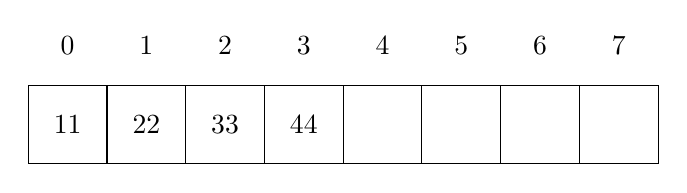
\begin{tikzpicture}
    \draw (0, 0) -- (8, 0);
    \draw (0, 1) -- (8, 1);
    \foreach \x in {0,...,8}
        \draw (\x, 0) -- (\x, 1);
    \foreach \x in {0,...,7}
        \node at (\x + 0.5, 1.5) {\x};

    \node at (0.5, 0.5) {11};
    \node at (1.5, 0.5) {22};
    \node at (2.5, 0.5) {33};
    \node at (3.5, 0.5) {44};
\end{tikzpicture}
\end{figure}

To see byte order in action, try this program:
\begin{wellcode}
    /* byte order: display bytes of a long */
    int main(void)
    {
        unsigned long x;
        unsigned char *p;
        int i;

        /* 11 22 33 44 => big-endian */
        /* 44 33 22 11 => little-endian */

        x = 0x11223344;
        p = (unsigned char *)&x;
        for (i = 0; i < sizeof(long); i++)
            printf("%x ", *p++);
        printf("\n");
        return 0;
    }
\end{wellcode}
On a 32-bit big-endian machine, the output is
\begin{wellcode}
    11 22 33 44
\end{wellcode}
but on a little-endian machine, it is
\begin{wellcode}
    44 33 22 11
\end{wellcode}
and on the PDP-11 (a vintage (古老的) 16-bit machine still found in
embedded systems), it is
\begin{wellcode}
    22 11 44 33
\end{wellcode}
On machines with 64-bit longs, we can make the constant bigger and see
similar behaviors.

This may seem like a silly (愚蠢的) program, but if we wish to send an
integer down a byte-wide interface such as a network connection, we need to
choose which byte to send first, and that choice is in essence (本质上) the
big-endian and little-endian decision. In other words, this program is
doing explicitly what
\begin{wellcode}
    fwrite(&x, sizeof(x), 1, stdout);
\end{wellcode}
does implicitly. It is not safe to write an \verb'int' (or \verb'short' or
\verb'long') from one computer and read it as an \verb'int' on another
computer.

For example, if the source computer writes with
\begin{wellcode}
    unsigned short x;
    fwrite(&x, sizeof(x), 1, stdout);
\end{wellcode}
and the receiving computer reads with
\begin{wellcode}
    unsigned short x;
    fread(&x, sizeof(x), 1, stdin);
\end{wellcode}
the value of \verb'x' will not be preserved if the machines have different
byte orders. If \verb'x' starts as \verb'0x1000' it may arrive as
\verb'0x0010'.

This problem is frequently solved using conditional compilation and "byte
swapping,"  something like this:
\begin{badcode}
    short x;
    fread(&x, sizeof(x), 1, stdin);
    #ifdef BIG_ENDIAN
    /* swap bytes */
    x = ((x&0xff) << 8) | ((x>>8) & 0xff);
    #endif
\end{badcode}
This approach becomes unwieldy (笨拙的) when many two-byte and four-byte
integers are being exchanged. In practice, the bytes end up being swapped
more than once as they pass from place to place.

If the situation is bad for \verb'short', it's worse for longer data types,
because there are more ways to permute (变更) the bytes. Add in the
variable padding between structure members, alignment restrictions, and the
mysterious byte orders of older machines, and the problem looks intractable
(棘手的).

\emph{Use a fixed byte order for data exchange.} There is a solution. Write
the bytes in a canonical order using portable code:
\begin{wellcode}
    unsigned short x;
    putchar(x >> 8);    /* write high-order byte */
    putchar(x & 0xff);  /* write low-order byte */
\end{wellcode}
then read it back a byte at a time and reassemble it:
\begin{wellcode}
    unsigned short x;
    x = getchar() << 8);    /* read high-order byte */
    x |= getchar() & 0xff;  /* read low-order byte */
\end{wellcode}

The approach generalizes to structures if you write the values of the
structure members in a defined sequence, a byte at a time, without padding.
It doesn't matter what byte order you pick; anything consistent will do.
The only requirement is that sender and receiver agree on the byte order in
transmission and on the number of bytes in each object. In the next chapter
we show a pair of routines to wrap up (掩饰) the packing and unpacking of
general data.

Byte-at-a-time processing may seem expensive, but relative to (涉及) the
I/O that makes the packing and unpacking necessary, the penalty (成本) is
minute. Consider the X Window system, in which the client writes data in
its native byte order and the server must unpack whatever the client sends.
This may save a few instructions on the client end, but the server is made
larger and more complicated by the necessity of handling multiple byte
orders at the same time -- it may well have concurrent big-endian and
little- endian clients -- and the cost in complexity and code is much more
significant.  Besides, this is a graphics environment where the overhead to
pack bytes will be swamped (淹没) by the execution of the graphical
operation it encodes.

The X Window system negotiates (协商) a byte order for the client and
requires the server to be capable of both. By contrast, the Plan 9
operating system defines a byte order for messages to the file server (or
the graphics server) and data is packed and unpacked with portable code, as
above. In practice the run-time effect is not detectable; compared to I/O,
the cost of packing the data is insignificant.

Java is a higher-level language than C or C++ and hides byte order
completely.  The libraries provide a \verb'Serializable' interface that
defines how data items are packed for exchange.

If you're working in C or C++, however, you must do the work yourself. The
key point about the byte-at-a-time approach is that it solves the problem
without \verb'#ifdef's, for any machines that have 8-bit bytes. We'll
discuss this further in the next chapter.

Still, the best solution is often to convert information to text format,
which (except for the CRLF problem) is completely portable; there is no
ambiguity about representation. It's not always the right answer, though.
Time or space can be critical, and some data, particularly floating point,
can lose precision due to roundoff (四舍五入) when passed through
\verb'printf' and \verb'scanf'. If you must exchange floating-point values
accurately, make sure you have a good formatted I/O library; such libraries
exist, but may not be part of your existing environment. It's especially
hard to represent floating-point values portably in binary, but with care,
text will do the job.

There is one subtle (微妙的) portability issue in using standard function
to handle binary file -- it is necessary to open such files in binary mode:
\begin{wellcode}
    FILE *fin;

    fin = fopen(binary_file, "rb");
    c = getc(fin);
\end{wellcode}

If the \verb"'b'" is omitted, it typically makes no difference at all on
Unix systems, but on Windows systems the first control-Z byte (octal
\verb'032', hex \verb'1A') of input will terminate reading (we saw this
happen to the strings program in Chapter \ref{chap:debug}). On the other
hand, using binary mode to read text files will cause \verb'\r' to be
preserved on input, and not generated on output.

\section{Portability and Upgrade}
\label{sec:portability_upgrade}

One of the most frustrating sources of portability problems is system
software that changes during its lifetime. These changes can happen at any
interface in the system, causing gratuitous (无理由的) incompatibilities
between existing versions of programs.

\emph{Change the name if you change the specification.} Our favorite (if
that is the word) example is the changing properties of the Unix
\verb'echo' command, whose initial design was just to echo its arguments:
\begin{wellcode}
    % echo hello, world
    hello, world
    %
\end{wellcode}
However, \verb'echo' became a key part of many shell scripts, and the need
to generate formatted output became important. So \verb'echo' was changed
to interpret its arguments, somewhat like \verb'printf':
\begin{wellcode}
    % echo 'hello\nworld'
    hello
    world
    %
\end{wellcode}
This new feature is useful, but causes portability problems for any shell
script that depends on the \verb'echo' command to do nothing more than
echo. The behavior of
\begin{wellcode}
    % echo BPATH
\end{wellcode}
now depends on which version of \verb'echo' we have. If the variable
happens by accident to contain a backslash, as may happen on DOS or
Windows, it may be interpreted by \verb'echo'. The difference is similar to
that between the output from \verb'printf(str)' and
\verb'printf("%s", str)' if the string \verb'str' contains a percent sign
(百分号).

We've told only a fraction of the full \verb'echo' story, but it
illustrates the basic problem: changes to systems can generate different
versions of software that intentionally behave differently, leading to
unintentional portability problems. And the problems are very hard to work
around. It would have caused much less trouble had the new version of
\verb'echo' been given a distinct name.

As a more direct example, consider the Unix command \verb'sum', which
prints the size and a checksum of a file. It was written to verify that a
transfer (转送) of information was successful:
% TODO: The "copy file to other_machine" should be italic.
\begin{wellcode}
    % sum file
    52313 2 file
    % copy file to other_machine
    %
    % telnet other_machine
    >
    > sum file
    52313 2 file
    >
\end{wellcode}
The checksum is the same after the transfer, so we can be reasonably
confident that the old and new copies are identical.

Then systems proliferated (扩散), versions mutated (变异), and someone
observed that the checksum algorithm wasn't perfect, so \verb'sum' was
modified to use a better algorithm.  Someone else made the same observation
and gave \verb'sum' a different better algorithm.  And so on, so that today
there are multiple versions of \verb'sum', each giving a different answer.
We copied one file to nearby machines to see what \verb'sum' computed:
% TODO: The "copy file to machine[23]" should be italic.
\begin{wellcode}
    % sum file
    52313 2 file
    % copy file to machine2
    % copy file to machine3
    % telnet machine2
    >
    > sum file
    eaa0d468 713 file
    > telnet  machine3
    >
    > sum file
    62992 1 file
    >
\end{wellcode}
Is the \verb'file' corrupted, or do we just have different versions of
\verb'sum'? Maybe both.

Thus \verb'sum' is the perfect portability disaster: a program intended to
aid in the copying of software from one machine to another has different
incompatible versions that render (给予) it useless for its original
purpose.

For its simple task, the original \verb'sum' was fine; its low-tech
(技术含量低) checksum algorithm was adequate. "Fixing" it may have made it
a better program, but not by much, and certainly not enough to make the
incompatibility worthwhile. The problem is not the enhancements but that
incompatible programs have the same name. The change introduced a
versioning problem that will plague (折磨) us for years.

\emph{Maintain compatibility with existing programs and data.} When a new
version of software such as a word processor is shipped, it's common for it
to read files produced by the old version. That's what one would expect: as
unanticipated (意外的) features are added, the format must evolve (演化).
But new versions sometimes fail to provide a way to write the previous file
format. Users of the new version, even if they don't use the new features,
cannot share their files with people using the older software and everyone
is forced to upgrade. Whether an engineering oversight (疏忽) or a
marketing strategy, this design is most regrettable (可悲的).

\textit{Backwards compatibility} is the ability of a program to meet its
older specification.  If you're going to change a program, make sure you
don't break old software and data that depend on it. Document the changes
well, and provide ways to recover the original behavior. Most important,
consider whether the change you're proposing is a genuine (真正的)
improvement when weighed against the cost of any non-portability you will
introduce.

\section{Internationalization}
\label{sec:internationalization}

If one lives in the United States, it's easy to forget that English is not
the only language, ASCII is not the only character set, \verb'$' is not the
only currency symbol, dates can be written with the day first, times can be
based on a 24-hour clock, and so on. So another aspect of portability,
taken broadly, deals with making programs portable across language and
cultural boundaries. This is potentially a very big topic, but we have
space to point out only a few basic concerns.

\textit{Internationalization} is the term for making a program run without
assumptions about its cultural environment. The problems are many, ranging
from character sets to the interpretation of icons in interfaces.

\emph{Don't assume ASCII.} Character sets are richer than ASCII in most
parts of the world.  The standard character-testing functions in
\verb'ctype.h' generally hide these differences:
\begin{wellcode}
    if (isalpha(c)) ...
\end{wellcode}
is independent of the specific encoding of characters, and in addition will
work correctly in locales where there are more or fewer letters than those
from \verb'a' to \verb'z' if the program is compiled in that locale. Of
course, even the name \verb'isalpha' speaks to its origins; some languages
don't have alphabets at all.

Most European countries augment (扩展) the ASCII encoding, which defines
values only up to \verb'Ox7F' (7 bits), with extra characters to represent
the letters of their language.  The Latin-1 encoding, commonly used
throughout Western Europe, is an ASCII superset that specifies byte values
from \verb'0x80' to \verb'0xFF' for symbols and accented (重音) characters;
\verb'0xE7', for instance, represents the accented letter \verb'c'. The
English word "boy" is represented in ASCII (or Latin-1) by three bytes with
hexadecimal values \verb'62 6F 79', while the French word "garcon" is
represented in Latin-1 by the bytes \verb'67 61 72 E7 6F 6E'. Other
languages define other symbols, but they can't all fit in the 128 values
left unused by ASCII, so there are a variety of conflicting standards for
the characters assigned to bytes \verb'0x80' through \verb'0xFF'.

Some languages don't fit in 8 bits at all; there are thousands of
characters in the major Asian languages. The encodings used in China,
Japan, and Korea all have 16 bits per character. As a result, to read a
document written in one language on a computer set up for another is a
major portability problem. Assuming the characters arrive intact
(原封不动地), to read a Chinese document on an American computer involves,
at a minimum, special software and fonts. If we want to use Chinese,
English, and Russian together, the obstacles are formidable (可怕的).

The Unicode character set is an attempt to ameliorate (改善) this situation
by providing a single encoding for all languages throughout the world.
Unicode, which is compatible with the 16-bit subset of the IS0 10646
standard, uses 16 bits per character, with values \verb'00FF' and below
corresponding to Latin-1. Thus the word "garcon" is represented by the
16-bit values \verb'0067 0061 0072 00E7 006F 006E', while the Cyrillic
(西里尔) alphabet occupies values \verb'0401' through \verb'04FF', and the
ideographic (表意的) languages occupy a large block starting at
\verb'3000'. All well-known languages, and many not so well-known, are
represented in Unicode, so it is the encoding of choice for transferring
documents between countries or for storing multilingual (多语言的) text.
Unicode is becoming popular on the Internet and some systems even support
it as a standard format; Java, for example, uses Unicode as its native
character set for strings. The Plan 9 and Inferno operating systems use
Unicode throughout, even for the names of files and users.  Microsoft
Windows supports the Unicode character set, but does not mandate (强制的)
it; most Windows applications still work best in ASCII but practice is
rapidly evolving towards Unicode.

Unicode introduces a problem, though: characters no longer fit in a byte,
so Unicode text suffers from the byte-order confusion. To avoid this,
Unicode documents are usually translated into a byte-stream encoding
called UTF-8 before being sent between programs or over a network. Each
16-bit character is encoded as a sequence of 1, 2, or 3 bytes for
transmission. The ASCII character set uses values \verb'00' through
\verb'7F', all of which fit in a single byte using UTF-8, so UTF-8 is
backwards compatible with ASCII. Values between \verb'80' and \verb'7FF'
are represented in two bytes, and values \verb'800' and above are
represented in three bytes. The word "garcon" appears in UTF-8 as the bytes
\verb'67 61 72 C3 A7 6F 6E'; Unicode value \verb'E7', the '\c{c}'
character, is represented as the two bytes \verb'C3 A7' in UTF-8.

The backwards compatibility of UTF-8 and ASCII is a boon (恩惠), since it
permits programs that treat text as an uninterpreted byte stream to work
with Unicode text in any language. We tried the \verb'Markov' programs from
Chapter \ref{chap:desipl} on UTF-8 encoded text in Russian, Greek,
Japanese, and Chinese, and they ran without problems. For the European
languages, whose words are separated by ASCII space, tab, or newline.  the
output was reasonable nonsense. For the others, it would be necessary to
change the word-breaking rules to get output closer in spirit (在精神上) to
the intent of the program.

C and C++ support "wide characters," which are 16-bit or larger integers
and some accompanying functions that can be used to process characters in
Unicode or other large character sets. Wide character string literals are
written as \verb'L"..."', but they introduce further portability problems:
a program with wide character constants can only be understood when
examined on a display that uses that character set.  Since characters must
be converted into byte streams such as UTF-8 for portable transmission
between machines. C provides functions to convert wide characters to and
from bytes. But which conversion do we use? The interpretation of the
character set and the definition of the byte-stream encoding are hidden in
the libraries and difficult to extract (抽取); the situation is
unsatisfactory (不令人满意的) at best (最多). It is possible that in some
rosy (理想的) future everyone will agree on which character set to use but
a likelier scenario (方案) will be confusion reminiscent (回忆) of the
byte-order problems that still pester (纠缠) us.

\emph{Don't assume English.} Creators of interfaces must keep in mind that
different languages often take significantly different numbers of
characters to say the same thing, so there must be enough room on the
screen and in arrays.

What about error messages? At the very least (最起码), they should be free
of jargon (术语) and slang (俚语) that will be meaningful only among a
selected population; writing them in simple language is a good start. One
common technique is to collect the text of all messages in one spot so that
they can be replaced easily by translations into other languages.

There are plenty of cultural dependencies, like the \verb'mm/dd/yy' date
format that is used only in North America. If there is any prospect (可能)
that software will be used in another country, this kind of dependency
should be avoided or minimized.  Icons in graphical interfaces are often
culture-dependent; many icons are inscrutable (难以理解的) to natives of
the intended environment, let alone (更不用说) people from other
backgrounds.

\section{Summary}

Portable code is an ideal that is well worth striving for, since so much
time is wasted making changes to move a program from one system to another
or to keep it running as it evolves and the systems it runs on changes.
Portability doesn't come for free, however. It requires care in
implementation and knowledge of portability issues in all the potential
target systems.

We have dubbed (轻点) the two approaches to portability union and
intersection.  The union approach amounts to (相当于) writing versions that
work on each target, merging the code as much as possible with mechanisms
like conditional compilation. The drawbacks are many: it takes more code
and often more complicated code, it's hard to keep up to date, and it's
hard to test.

The intersection approach is to write as much of the code as possible in a
form that will work without change on each system. Inescapable (不可避免的)
system dependencies are encapsulated in single source files that act as an
interface between the program and the underlying system. The intersection
approach has drawbacks too, including potential loss of efficiency and even
of features, but in the long run, the benefits outweigh the costs.

\section*{Supplementary Reading}

There are many descriptions of programming languages, but few are precise
enough to serve as definitive references. The authors admit to a personal
bias towards \bookname{The C Programming Language} by Brian Kernighan and
Dennis Ritchie (Prentice Hall, 1988), but it is not a replacement for the
standard. Sam Harbison and Guy Steele's \bookname{C: A Reference Manual}
(Prentice Hall, 1994), now in its fourth edition, has good advice on C
portability. The official C and C++ standards are available from ISO, the
International Organization for Standardization. The closest thing to an
official standard for Java is \bookname{The Java Language Specification},
by James Gosling, Bill Joy, and Guy Steele (Addison-Wesley, 1996).

Rich Stevens's \bookname{Advanced Programming in the Unix Environment}
(Addison-Wesley, 1992) is an excellent resource for Unix programmers, and
provides thorough coverage of portability issues among Unix variants.

POSIX, the Portable Operating System Interface, is an international
standard defining commands and libraries based on Unix. It provides a
standard environment, source code portability for applications, and a
uniform interface to I/O, file systems and processes. It is described in a
series of books published by the IEEE.

The term "big-endian" was coined by Jonathan Swift in 1726. The article by
Danny Cohen, "On holy wars and a plea (请求) for peace," \bookname{IEEE
Computer}, October 1981, is a wonderful fable (寓言) about byte order
that introduced the "endian (尾端)" terms to computing.

The Plan 9 system developed at Bell Labs has made portability a central
priority.  The system compiles from the same \verb'#ifdef'-free source on a
variety of processors and uses the Unicode character set throughout. Recent
versions of Sam (first described in "The Text Editor sam,"
\bookname{Software -- Practice and Experience, 17, l1}, pp. 813-845, 1987)
use Unicode, but run on a wide variety of systems. The problems of dealing
with 16-bit character sets like Unicode are discussed in the paper by Rob
Pike and
Ken Thompson, "Hello World or\footnote{Unrecognized characters.}"
\bookname{Proceedings of the Winter 1993 USENIX Conference}, San Diego,
1993, pp. 43-50. The UTF-8 encoding made its first appearance in this
paper. This paper is also available at the Plan 9 web site at Bell Labs, as
is the current version of Sam.

The Inferno system, which is based on the Plan 9 experience, is somewhat
analogous to Java, in that it defines a virtual machine that can be
implemented on any real machine, provides a language (Limbo) that is
translated into instructions for this virtual machine, and uses Unicode as
its native character set. It also includes a virtual operating system that
provides a portable interface to a variety of commercial systems. It is
described in "The Inferno Operating System," by Sean Dorward, Rob Pike,
David Leo Presotto, Dennis M. Ritchie, Howard W. Trickey, and Philip
Winterbottom, \bookname{Bell Labs Technical Journal, 2, 1}, Winter, 1997.
